%  ========================================================================
%  Copyright (c) 1985 The University of Washington
%
%  Licensed under the Apache License, Version 2.0 (the "License");
%  you may not use this file except in compliance with the License.
%  You may obtain a copy of the License at
%
%      http://www.apache.org/licenses/LICENSE-2.0
%
%  Unless required by applicable law or agreed to in writing, software
%  distributed under the License is distributed on an "AS IS" BASIS,
%  WITHOUT WARRANTIES OR CONDITIONS OF ANY KIND, either express or implied.
%  See the License for the specific language governing permissions and
%  limitations under the License.
%  ========================================================================
%

% Documentation for University of Washington thesis LaTeX document class
% by Jim Fox
% fox@washington.edu
%
%    Revised 2020/02/24, added \caption()[]{} option.  No ToC.
%
%    Revised for version 2015/03/03 of uwthesis.cls
%    Revised, 2016/11/22, for cleanup of sample copyright and title pages
%
%    This document is contained in a single file ONLY because
%    I wanted to be able to distribute it easily.  A real thesis ought
%    to be contained on many files (e.g., one for each chapter, at least).
%
%    To help you identify the files and sections in this large file
%    I use the string '==========' to identify new files.
%
%    To help you ignore the unusual things I do with this sample document
%    I try to use the notation
%
%    % --- sample stuff only -----
%    special stuff for my document, but you don't need it in your thesis
%    % --- end-of-sample-stuff ---


%    Printed in twoside style now that that's allowed
%

\documentclass [11pt, proquest] {uwthesis}[2020/02/24]

%
% The following line would print the thesis in a postscript font

% \usepackage{natbib}
% \def\bibpreamble{\protect\addcontentsline{toc}{chapter}{Bibliography}}

\setcounter{tocdepth}{1}  % Print the chapter and sections to the toc


% ==========   Local defs and mods
%

% --- sample stuff only -----
% These format the sample code in this document

\usepackage{alltt}  %
\newenvironment{demo}
  {\begin{alltt}\leftskip3em
     \def\\{\ttfamily\char`\\}%
     \def\{{\ttfamily\char`\{}%
     \def\}{\ttfamily\char`\}}}
  {\end{alltt}}

% metafont font.  If logo not available, use the second form
%
% \font\mffont=logosl10 scaled\magstep1
\let\mffont=\sf
% --- end-of-sample-stuff ---

\usepackage{natbib}
\usepackage[colorlinks,linkcolor=blue,citecolor=blue,urlcolor=blue,bookmarks=false,hypertexnames=true]{hyperref}
\usepackage{booktabs}
\usepackage{arydshln}

\usepackage{graphicx}
%\graphicspath{ {./images/} }


\begin{document}

% ==========   Preliminary pages
%
% ( revised 2012 for electronic submission )
%

% \prelimpages

%
% ----- copyright and title pages
%
\Title{“Obama never said that”: Evaluating fact-checks for topical consistency and quality }
\Author{Katya Simpson}
\Year{2022}
\Program{Department of Linguistics}

\Chair{Name of Chairperson}{Title of Chair}{Department of Chair}
\Signature{First committee member}


\copyrightpage

\titlepage


%
% ----- signature and quoteslip are gone
%

%
% ----- abstract
%


\setcounter{page}{-1}
\abstract{

I need to write this!

%
% This sample dissertation is an aid to students who are attempting
% to format their theses with \LaTeX, a sophisticated
% text formatter widely used by mathematicians and scientists everywhere.

% \begin{itemize}
% \item It describes the use of a specialized
% macro package developed specifically for thesis production
% at the University.
% The macros customize \LaTeX\ for the correct thesis style,
% allowing the student to concentrate on the substance of
% his or her text.%
% \footnote{See Appendix A to obtain the source to this
%  thesis and the class file.}
% \item It demonstrates the solutions to a variety of
% formatting challenges found in thesis production.
% \item It serves as a template for a real dissertation.
% \end{itemize}
}

%
% ----- contents & etc.
%
\tableofcontents
\listoffigures
%\listoftables  % I have no tables

%
% ----- glossary
%
% \chapter*{Glossary}      % starred form omits the `chapter x'
% \addcontentsline{toc}{chapter}{Glossary}
% \thispagestyle{plain}
% %
% \begin{glossary}
% \item[argument] replacement text which customizes a \LaTeX\ macro for
% each particular usage.
% \item[back-up] a copy of a file to be used when catastrophe strikes
% the original.  People who make no back-ups deserve
% no sympathy.
% \item[control sequence] the normal form of a command to \LaTeX.
% \item[delimiter] something, often a character, that indicates
% the beginning and ending of an argument.
% More generally, a delimiter is a field separator.
% \item[document class] a file of macros that tailors \LaTeX\ for
% a particular document.  The macros described by this thesis
% constitute a document class.
% \item[document option] a macro or file of macros
% that further modifies \LaTeX\ for
% a particular document.  The option {\tt[chapternotes]}
% constitutes a document option.
% \item[figure] illustrated material, including graphs,
% diagrams, drawings and photographs.
% \item[font] a character set (the alphabet plus digits
% and special symbols) of a particular size and style.  A couple of fonts
% used in this thesis are twelve point roman and {\sl twelve point roman
% slanted}.
% \item[footnote] a note placed at the bottom of a page, end of a chapter,
% or end of a thesis that comments on or cites a reference
% for a designated part of the text.
% \item[formatter] (as opposed to a word-processor) arranges printed
% material according to instructions embedded in the text.
% A word-processor, on the other hand, is normally controlled
% by keyboard strokes that move text about on a display.
% \item[\LaTeX] simply the ultimate in computerized typesetting.
% \item[macro]  a complex control sequence composed of
% other control sequences.
% \item[pica] an archaic unit of length.  One pica is twelve points and
% six picas is about an inch.
% \item[point] a unit of length.  72.27 points equals one inch.
% \item[roman]  a conventional printing typestyle using serifs.
% the decorations on the ends of letter strokes.
% This thesis is set in roman type.
% \item[rule] a straight printed line; e.g., \hrulefill.
% \item[serif] the decoration at the ends of letter strokes.
% \item[table] information placed in a columnar arrangement.
% \item[thesis] either a master's thesis or a doctoral dissertation.
% This document also refers to itself as a thesis, although it
% really is not one.

% \end{glossary}

%
% ----- acknowledgments
%
\acknowledgments{% \vskip2pc
  % {\narrower\noindent
  Put my acknowledgements here!
  % \par}
}

%
% ----- dedication
%
\dedication{\begin{center} write dedication here \end{center}}

%
% end of the preliminary pages



%
% ==========      Text pages
%

\textpages

% ========== Chapter 1

\chapter {Introduction}

Write me. Put RQs and also why were using Sia et al over LDA

% The utility of a clean, professionally prepared thesis is well
% documented%
% \footnote{See, for example,
%   W.~Shakespeare\cite{Hamlet} for a recent discussion.}
% and, even if you never intend to actually print your thesis,
% you still ought to format it as if that were your intention.

% \TeX\ facilitates that. It is a flexible,
% complete and professional typesetting system.
% It will produce {\bf pdf} output as required by the Graduate School.

% \section{The Purpose of This Sample Thesis}

% This sample is both a demonstration of the quality and
% propriety of a \LaTeX formatted thesis and
% documentation for its preparation.
% It has made extensive use of a custom class file
% developed specifically for this purpose
% at the University of Washington.  Chapter~II discusses
% \TeX\ and \LaTeX.
% Chapter III describes the additional macros and functions
% provided by the custom thesis class file.  Finally, Chapter IV hopes to tie things up.

% It is
% impossible to predict all the formatting problems one will encounter
% and there will be problems that are best handled
% by a specialist.
% The Graduate School may be able to help you find help.
% Some departments may also be able to provide \LaTeX\ assistance.


% \section{Conventions and Notations}

% In this thesis the typist
% refers to the user of \LaTeX---the one who
% makes formatting decisions and chooses the appropriate
% formatting commands.
% He or she will most often be the degree candidate.

% This document deals with \LaTeX\ typesetting commands and their
% functions.  Wherever possible the conventions used to display
% text entered by the typist and the resulting formatted output
% are the same as those used by the \TeX books.
% Therefore, {\tt typewriter type} is used to indicate text
% as typed by the computer
% or entered by the typist.
% It is quite the opposite of {\it italics,} which indicates
% a category rather than exact text.  For example,
% {\tt alpha} and {\tt beta} might each be an example of a {\it label}.


% \section{Nota bene}

% This sample thesis was produced by the \LaTeX\ document class it describes
% and its format is consonant with the Graduate School's electronic dissertation guidelines,
% as of November, 2014, at least.
% However, use of this package does not guarantee acceptability
% of a particular thesis.


% ========== Chapter 2

\chapter{Literature Review}

We apply methods from natural language processing (NLP) to the misinformation fact-checking space, and look to three areas to guide and ground our work.  Within NLP literature, we look at alternatives to  Latent Dirichlet Allocation (LDA) \cite{blei2003latent} and at topic modeling as it relates to fact-checking. We also learn from studies on Twitter's Birdwatch program within the fact-checking and misinformation literature.

\section{Alternatives to LDA}

 \cite{sia-etal-2020-tired} introduce a computationally-efficient alternative to classical topic models like LDA. The key theoretical addition in their work is to think of  topics as “clusters of word types” where word types can be represented by embeddings.  They tested different clustering techniques, using contextualized and non-contextualized embeddings, and incorporating  corpus statistics. They found that using term-frequency weighted KMeans clustering (with reranking of top word types with term-frequencies) yields topics that are comparably coherent to those generated with LDA.

 \cite{chen2016short} and \cite{pang2016mr} note the difficulties of using LDA on short documents because of the heavy noise and lack of sufficient word co-occurrences. They propose methods to modify LDA, primarily as part of classification tasks.

MOVE ME TO INTO?
 Given the computational-efficiency and relative simplicity of the method proposed by \cite{sia-etal-2020-tired}, it seems to be a good fit for the fast-moving fact-checking space.

 \section{Topic Modeling and Fact-Checking}
 Elements of topic modeling has been applied to automatic fact verification. \cite{si-etal-2021-topic} propose a model that checks for topical consistency (using LDA) between a claim and pieces of evidence, and classifies the evidence as supporting or refuting the claim. \cite{Hardalov2021ASO}, in a survey paper on stance detection (often used in fact-checking tasks),  note that the benefits of using unsupervised topic models are limited because they tend to be noisy. \cite{hanselowski-etal-2018-retrospective} evaluates methods in a Fake News Challenge and found that methods that used features from topic models did not capture semantic relationships necessary to do well on the task. These challenges emphasize the need to evaluate new topic modeling methods in the fact-checking area.

 As far as the author is aware, this thesis is the first attempt to use the method introduced by \cite{sia-etal-2020-tired} in a fact-checking context. This thesis is also limited in comparison to the goals usually seen in fact-checking literature: we aim to learn about topic overlap between content and crowd-sourced fact-checks, not to classify the content.

 \section{Background on Twitter's Birdwatch}

Twitter introduced Birdwatch in 2021 \citep{coleman_2021} in an effort to identify and annotate misinformation on their platform. Birdwatch is community-based and relies on users to perform three mechanisms: labelling tweets as \verb|misleading| or \verb|not misleading|, writing annotations (``notes") for tweets, and rating each other's notes for quality. The data generated from these mechanisms is freely available in the US on the \href{https://twitter.github.io/birdwatch/}{Birdwatch User Guide}.

This thesis refers to the Birdwatch program and
the Birdwatch dataset. The Birdwatch program is
what a Birdwatch user would interact with when
they log on to Twitter and is the primary design
focus of the Twitter Birdwatch team. The dataset is
the output of the program: the data generated by
users writing and rating notes.

The Birdwatch dataset has not been widely studied in the NLP community, likely because of how new and relatively small it is (though the widespread analysis of Twitter's tweet data \citep{antonakaki2021survey} may indicate that the Birdwatch dataset will inevitably also be analyzed at scale). It has been evaluated from a security standpoint, examining sociotechnical vulnerabilities of the program \citep{benjamin2021watches}. The benefits and pitfalls of crowd-sourced fact-checking for Birdwatch have been studied by \cite{yasseri2021can}. \cite{allen2021birds} used Birdwatch data in an experiment that found that partisanship of Birdwatch users is highly correlated with the type of notes they write. The crowd-sourced nature of Birdwatch, and the many design considerations that are necessary for good social media data use, are briefly examined in the Ethical Considerations section (\ref{ethicalconsiderations}).





\chapter{Methodology}

We replicate the method from \cite{sia-etal-2020-tired}, with some modifications, to create clusters of word types from the Birdwatch corpus and treat those clusters as learned topics.

\section{Birdwatch Terminology}

% why is this space here?

\begin{itemize}
\item \textbf{Note}: a fact-checking annotation that is in response to a tweet. Notes usually include linked sources
\item \textbf{Tweet}: we think of tweets as the ``sister" document (or ``claim") that a note references. A tweet can have multiple notes.
\item \textbf{Rating}: users can mark a note as ``Helpful", ``Somewhat Helpful", or ``Not Helpful" and label it with several other tags. The rating system is an effort to maintain the quality of notes. It allows the Birdwatch program to hide largely unhelpful notes and emphasize very helpful notes in Twitter's user interface. A note can have multiple ratings.
\end{itemize}

The term ``document" is used to refer to both notes and tweets.


\section{Data Collection and Preprocessing}\label{section:preprocessing}

The data was downloaded from the \href{https://twitter.github.io/birdwatch/download-data/}{Birdwatch github site} as two TSV files (one for notes and one for ratings) that includes data up to Jan 30th, 2022. This represents nearly a full year’s of data since the Birdwatch program was launched \cite{coleman_2021}. The notes data contains tweet IDs that map to the to the tweets being fact-checked. The DocNow hydrator \citep{docnow_hydrator} is used to obtain the tweet metadata (including the text) from the list of tweet IDs in accordance with Twitter’s use of service terms. Maintaining the mapping of a note and its associated tweet is not necessary while generating and clustering the embeddings but will be when testing for the topic overlap between the notes and tweets in the Experiment section \ref{section:experiments}.

Birdwatch was piloted in the US and most of the notes are written in English, although they could fact-check a non-English tweet. Later on in this method, a BERT model pre-trained on English \citep{DBLP:journals/corr/abs-1810-04805} will be used to generate embeddings for the documents . Thus, a minority of tweets without the English metadata labels were omitted. In the future, a multilingual approach could be used.

The documents are lower-cased with usernames, hashtags, urls, and digits omitted. The preprocessing step returns two outputs for each document: (1) a cleaned string that will be used by BERT (2) and a list of cleaned tokens with stopwords omitted that will be used to calculate corpus statistics. The first output  is a departure from the method outlined by \cite{sia-etal-2020-tired}, who omitted stopwords prior to generating the BERT embeddings. \cite{Qiao2019UnderstandingTB} find that omitting stopwords does not harm the performance of a BERT ranking task although they receive as much attention as non-stopwords. We use that finding to assume that BERT is ambivalent to stop-word removal and leave them in for this task because of the short document length of tweets and notes, hoping to get higher context embeddings. We remove stopwords prior to calculating term-frequencies in \ref{section:corpusstats} because we want to cluster over a meaningful vocabulary to create topics.

\section{Train/Test Split}\label{section:traintest}
We use a 60/40 train/test split. The train data is used to calculate corpus statistics and generate the word type embeddings, which are then clustered. The test data is used to evaluate the output of the train data clusters for topic coherence. The test/train split is necessary because the output topics are generated with term-frequency statistics and the primary evaluation method (Normalized PMI) will also depend on term-frequency statistics

\section{Corpus Statistics}\label{section:corpusstats}
Term frequencies (which will be used as weights while clustering word type embeddings) are calculated from the train data, using both notes and tweets to create the vocabulary. \cite{sia-etal-2020-tired} found that term frequencies (tf) are the most successful corpus statistics for this purpose and we follow their standard definition: $$ \textbf{tf} = \frac{n_t}{\Sigma_{t'}n_{t'}} $$  where $n_t$ is the count of a word type $t$. The final vocabulary size contains 23,090 word types.

\section{Generating BERT Embeddings}{section:embeddings}
Token embeddings are created using the BERT base model \cite{DBLP:journals/corr/abs-1810-04805}  (\verb|bert-base-uncased| pipeline from Huggingface).
A full note or tweet is used as the context window and the last hidden layer is taken as the token’s embedding. Following the method from \cite{sia-etal-2020-tired}, subword representations are averaged. This method can generate different embeddings for the identical tokens because of their different context windows. These word token embeddings are averaged to create word type embeddings.

\section{Clustering}\label{section:clustering}

The final step to find topics is to cluster the word type embeddings. \cite{si-etal-2021-topic} found that using the KMeans algorithm with term frequency weights to create the clusters, and using the weights to re-rank the top word types is effective. Prior to clustering, they also use PCA to reduce dimensions of the embeddings, noting that the method allows for significant dimension reductions (up to 80\%). This step is primarily to reduce the computational complexity of the process. Their method is followed: we use the tf weights calculated in \ref{section:corpusstats} with the KMeans algorithm \citep{scikit-learn}, and re-rank the word types in each cluster according to tf weights to find the most representative top word types.

Two hyperparameters are considered: the number of clusters for the KMeans algorithm (the number of topics) and the number of dimensions for PCA reduction.

Steps \ref{section:preprocessing} - \ref{section:clustering} ran over
\begin{itemize}
  \item 20, 50, and 100 clusters
  \item 100, 300, 500, and 768 (no PCA) dimensions
  \item Three random seeds to initialize the KMeans algorithm
\end{itemize}

The top ten words of the the first cluster generated (with twenty total clusters, one hundred dimensions, and  random seed = 372 ) are: ``us", ``country", ``central", ``north", ``national", ``state", ``american", ``usa", ``city", and ``nation".

\chapter{Evaluation of Topic Clusters}

In order to evaluate the coherence of the generated topic clusters, we follow \cite{sia-etal-2020-tired} and use Normalized Pointwise Mutual Information (NPMI) \citep{bouma2009normalized}.   NPMI is defined as $$\textbf{NPMI}(x,y) = \frac{\ln\frac{p(x,y)}{p(x)p(y)}}{-\ln(p(x,y))}$$

where $p(x)$ and $p(y)$ correspond to the probability of seeing words $x$ and $y$, and $p(x,y)$ correspond the probability of words co-occuring. The probabilities are calculated from the test data. We calculate NPMI for  the top 10 words for each cluster over each permutation of hyperparameters. The window for the PMI calculation indicates if it will capture a syntactic or semantic relationship \citep{jurafsky_martin_2019}. We use the first quartile of note length (14 tokens) as the window; intending to capture semantic relationship. The NPMI scores are averaged over three random seeds.  NPMI has a range from [-1,1] where 1 would indicate that two words only occur together and -1 indicates that they would be completely independent of each other.

NPMI is a metric based on vector semantics and provides a measure of similarity based on how often words co-occur. It has been found to correlate to human judgements \citep{lau2014machine} . However, it's also possible to evaluate clusters with alternative metrics that aren't based on word co-occurrence. We look into a distance-based internal clustering validation method, hoping to  reinforce any findings from the NPMI method. We include silhouette scores \citep{liu2010understanding}  to capture how far a top word’s embedding is to its cluster centroid and how far it is to other cluster's centroids. Similar to NPMI, it has a range from [-1,1] where -1 indicates that the top word may be in between or belong to several clusters, 0 indicates that there are overlapping clusters, and 1 indicates that the top word is perfectly contained in one distinct cluster. The mean score is then calculated over all the top words in a cluster  \citep{scikit-learn}.


\begin{table}
\centering
\caption{Evaluation Scores (averaged over three random seeds)}
\begin{tabular}{rrrr}
\toprule
 NClusters &  NDims &  NPMI\_Score &  Silhouette\_Index \\
\midrule
        20 &    100 &       -0.65 &              0.04 \\
        20 &    300 &       -0.67 &              0.06 \\
        20 &    500 &       -0.66 &              0.05 \\
        20 &    768 &       -0.62 &              0.06 \\
        50 &    100 &       -0.78 &              0.04 \\
        50 &    300 &       -0.73 &              0.05 \\
        50 &    500 &       -0.73 &              0.05 \\
        50 &    768 &       -0.72 &              0.05 \\
       100 &    100 &       -0.81 &              0.04 \\
       100 &    300 &       -0.76 &              0.04 \\
       100 &    500 &       -0.75 &              0.04 \\
       100 &    768 &       -0.73 &              0.04 \\
\bottomrule
\end{tabular}
\label{fig:Cluster_Evaluation}
\end{table}



The evaluation metrics are presented in Table \ref{fig:Cluster_Evaluation}. The NPMI scores are all negative which makes sense when we consider how short the documents are and how few (approximately 15,000) are available in the test set. High joint probabilities p(x,y) are relatively scarce and often are 0.  That is to say, the words exist separately but don’t occur together, resulting in an NPMI score of -1. This isn't entirely unexpected. It aligns with known problems about LDA which also suffers from sparse word co-occurrences when used on short social media text \citep{chen2016short}, \citep{pang2016mr}.

As an example, we can look at the NPMI scores for a fake cluster of words that should intuitively be highly correlated with each other. Consider [``biden", ``putin", ``russia", ``usa"]. We see that the pairwise NPMI is relatively low (Table \ref{fig:Missing_Pairs}), with the average being pulled to -1 because “putin” and “usa” don’t co-occur in the test set

\begin{table}
\centering
\caption{NPMI with missing co-occurrences}
\begin{tabular}{llr}
\toprule
    w1 &     w2 &  NPMI \\
\midrule
 biden &  putin &              0.16 \\
 biden & russia &              0.05 \\
 biden &    usa &              0.03 \\
 putin & russia &              0.29 \\
 putin &    usa &             -1.00 \\
russia &    usa &              0.12 \\
   usa &  biden &              0.01 \\
\bottomrule
\end{tabular}
\label{fig:Missing_Pairs}
\end{table}

The silhouette scores in Table \ref{fig:Cluster_Evaluation}  are close to zero because of high dimensionality of the data. \cite{kriegel2009clustering} note that one of the problems with evaluating clusters in high dimensions is that the concept of distance becomes less meaningful.  Interpreting distance metrics in high dimensions is a known problem \cite{tomavsev2016clustering} and limit the usefulness of silhouette indices and other distance based metrics.

Assuming that NPMI will have a baseline of close to -1; we take the permutation of hyperparameters that results in the highest NPMI (which, perhaps coincidentally, has the the highest silhouette score) and use 20 clusters and 768 dimensions.

Topic clusters (and all of their constituent word type embeddings) are re-generated with these parameters for analysis of the research questions. PCA is not used but should be re-considered if computational complexity becomes more of a concern (for example, if Birdwatch is more widely used and the dataset becomes much larger).

\chapter{Experiments and Analysis} \label{section:experiments}

\section{Research Question 1}

\textbf{Do notes that have high topic overlap with their associated tweet get better ratings?
}


Topic overlap is defined as the similarity between a tweet’s topic probability distribution and a note’s topic probability distribution. \cite{sia-etal-2020-tired} propose an extension to their method to find the top topics per document, which is slightly modified for this analysis. Using the word type embeddings,  the pairwise cosine similarity between each token in a document and cluster centroid is calculated. The token similarities are summed over the clusters to create a document similarity vector. This vector is then normalized with a softmax function yielding a probability distribution for the document over the possible topics.

Kullback–Leibler (KL) divergence is used to measure topic overlap using the document probability distributions. KL divergence captures the average number of extra bits required to encode a note’s topic distribution N using code optimized for a tweet’s topic distribution \citep{Murphy2012}. More generally, it represents the average amount of information needed to discriminate between N and T. It is not a symmetric measure. $KL(N || T)$ represents the case where the probability distribution of the note is compared to the tweet’s (or, how many average bits of information it would take to encode the note with code optimized for a tweet) . This direction intuitively captures the research question where the note is a response to a tweet, and is expected to have something in common with it. For a complete analysis, both directions will be computed. For a “yes” answer to RQ1, a negative relationship is expected: if the KL divergence is high, then the topic distributions are dissimilar, and helpfulness would be low. KL divergence was calculated with SciPy \citep{2020SciPy-NMeth}.

The other side of the research question is about ratings. Birdwatch provides user generated ratings in two categories. The \verb|helpful| category has two choices “Helpful” and “Not Helpful”. The \verb|helpfulnessLevel| category, added later to Birdwatch according to the user guide, has three choices “Helpful”, “Somewhat Helpful”, and “Not Helpful”. These options are mapped to numeric counterparts (-1, 0, 1) and the outcome variable for this analysis is defined as the average of the numeric counterparts for a note. It should be noted that note/tweet pairs created before the launch of the \verb|helpfulnessLevel| category may have a slightly different distribution in comparison to pairs created after the launch, but the effect of this is left to further research.
Finally, the helpfulness level of the notes  is linearly regressed against KL divergence of note/tweet pairs. Robust standard errors are used because the outcome variable is not normal.
The results are in Table \ref{fig:RQ1_OLS}.

\begin{table}
\centering
\caption{Regression Results with Document Length Limits ($\dagger$ denotes  p $< 0.001$)}
\begin{tabular}{lrrr}
\toprule
Regressor &  Note Min &  Tweet Min &   Coef(SE) \\
\midrule
    KL($N || T$) &         0 &          0 & $-0.291(0.051)^{\dagger$} \\
    KL($T || N$) &         0 &          0 & $-0.050(0.053)$ \\ \hdashline
    KL($N || T$) &         8 &          8 & $-0.051(0.098)$ \\
    KL($T || N$) &         8 &          8 &  $0.056(0.104)$ \\ \hdashline
    KL($N || T$) &         0 &          8 & $-0.377(0.055)^\dagger$ \\
    KL($T || N$) &         0 &          8 & $-0.293(0.083)^\dagger$ \\\hdashline
    KL($N || T$) &         8 &          0 & $-0.056(0.082)$ \\
    KL($T || N$)  &         8 &          0 &  $0.006(0.058)$ \\
\bottomrule

\end{tabular}
\label{fig:RQ1_OLS}
\end{table}


The relationship between helpfulness and $KL(N \|T)$ is statistically significant and negative.

Document length has a strong effect on this analysis. If a document has a low amount of words, the document similarity vector (the summed cosine similarity between tokens and cluster centroids) will be flattened because of the low information content. We can gain intuition for this by looking at the uniformity of the distribution by document length. KL divergence from a uniform distribution is calculated for each document’s topic distribution.There is a clear trend in Fig \ref{fig:uniform}, for both notes and tweets, that shows that shorter documents are more similar to the uniform distribution.

\begin{figure}[h]
\centering
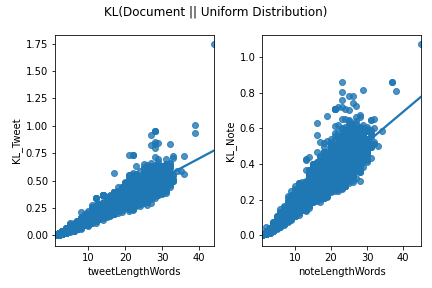
\includegraphics[scale=0.6]{KLUniform.png}
\caption{Uniformity as a function of length}
\label{fig:uniform}
\end{figure}

A uniform distribution for possible topics suggests that this topic model method is not well suited for short documents: it fails to return the top topics per document. If we omit “short” tweets (below the first quartile without stopwords, or 8 tokens), the relationship between KL divergence and helpfulness becomes statistically significantly negative for the tweet to note direction as well. Interestingly, this is not the case when short notes are omitted. This could be because helpful notes may add extra context, modifying the topic distribution. This line of reasoning is continued in the analysis of RQ 2 in section \ref{section:RQ2}.

We also tried a model specification geared towards separately identifying the impact of the KL distance between notes and tweets and the length of both the notes and the tweets on the helpfulness level. This model showed:

\begin{itemize}
    \item that the KL distance was still a statistically-significant predictor of the helpfulness in the presence of the other features
    \item that there was no heterogeneous effect. The KL distance interactions with either note length or tweet length were not statistically significant. This tells us that tweet and note lengths don’t strengthen the relationship between the Kullback-Leibler distance and the helpfulness.

\end{itemize}

 \section{Research Question 2}\label{section:RQ2}

\textbf{Can this method capture the helpful extra context that Birdwatch notes add to a tweet?}

Birdwatch users can label notes in a variety of ways after marking them as helpful (see figure \ref{fig:labels} as an example). Labels are not required to submit a rating so we make the assumption that the presence of at least one label per note is enough to associate the label’s trait with that note. For example, a note may have only one “Easy to Understand” label even though it has multiple ratings.



Intuitively, we can think of a note's extra context as a shift in the topic probability distribution when compared to its tweet. Figure \ref{fig:highcontext} shows an example.

\begin{figure}[h]
\centering
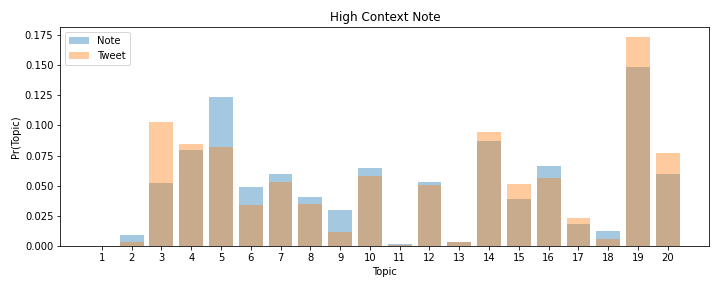
\includegraphics[scale=0.6]{HighContext.png}
\caption{This note was labeled as helpful because it adds important context. There is a shift in its topic distribution in comparison to the tweet }
\label{fig:highcontext}
\end{figure}

This research question will also be addressed using document topic probability distributions and focus on $KL(N || T)$ because it more clearly captures the note-tweet relationship. We try to approach the question from three different angles.

First, we find a subset of the data with \verb|Provide Important Context| labels and ask ``Will helpfulness increase as $KL(N || T)$ increases?" $$helpfulness \sim KL(N || T)$$ This is the same linear regression that was used in RQ1 but on subset of the original data. The result is statistically significant and negative: if the topics are similar then helpfulness still increases.  However, the coefficient is lower than when calculated over the entire dataset (row 1 of Table Y). Being on-topic is a less strong lever for helpfulness when considering notes marked with the “Provides Important Context” label.

Second, we return to considering the entire dataset and ask ``Does the presence of the add context label increase the effect of $KL(N || T)$ on helpfulness?" $$helpfulness \sim KL(N || T) + context\_add + KL(N || T) \times context\_add$$ We find that the addition of the \verb|Provides Important Context| label is not a strong lever and there are no heterogeneous effects.

Third, we continue to consider the entire dataset and ask ``What is the effect of $KL(N || T)$ on the probability of having add context label?". $$context\_add \sim KL(N || T)$$ The label's presence is a binary variable so a logistic regression is used and we find that there is not a statistically significant effect.

Birdwatch's rating mechanisms are not complete from an annotation perspective. The lack of certain label cannot be a indicator that the label truly does not apply. Certain notes may be labeled as adding context but it's very possible that there is a large proportion of notes that do indeed add context but have not been labeled as such. This casts some doubt on non-significant results from the second and third lines of inquiry which assume that $context\_add$ is binary variable that reflects the ground truth.

% RQ2 is approached in a similar way to  use the “Provides Important Context” label to find a subset of the documents where the notes helpfully add context to the tweet’s subject matter.

% Similar to the experiment for RQ1, this RQ can be addressed using document topic probability distributions. We focus on KL(N || T) because it more intuitively captures the notes and tweet relationship. The helpfulness level of the notes is linearly regressed against KL divergence of note/tweet pairs in the two data subsets.

% INSERT TABLE HERE

% The result is statistically significant and negative: if the topics are similar then helpfulness still increases.  However, the coefficient is lower than the original dataset: being on-topic is a less strong lever for notes marked with the “Provides Important Context” label.

Finally,  we return to the question posed in RQ1 and evaluate if the average length of the notes differs between the ones with context-adding  labels and the ones without, using a two-sided t-test. It yields a t-statistic of statistic=-10.985 with a p-value $< 0.0001$. That is, the context adding subset has statistically significantly longer notes than the notes that don’t have that label. This adds some credence to interpretation from RQ1: omitting short notes leads to an insignificant relationship between KL divergence and helpfulness because longer notes may add context and shift the topic distribution. Note that the caveat about Birdwatch's incomplete annotations applies to this analysis as well.

\chapter{Discussion}

We find a statistically significant negative relationship between the independent variable KL(N || T) and the dependent variable (helpfulness). The answer to RQ1 is yes: notes that have higher topic overlap with their tweets seem to get better, or more helpful, ratings. The directionality of KL divergence plays a role in this interpretation. While KL(N || T) was found to be a statistically significant variable, KL(T || N) was not. One possible explanation is that notes can add context to the tweet’s original content and alter the document’s topic distribution. Then, the additional average information to encode a tweet (based on code optimized for the note) would increase to accommodate the topic distribution shift.

Omitting short tweets results in a stronger relationship between KL(N || T) and helpfulness, and a statistically significant relationship with KL(T || N). However, omitting short notes results in no significant relationships at all. A possible explanation for this is that longer notes may add more context than short notes (intuitively, it would take more tokens to both address the tweet’s topic and add in new context to refute or support it). This explanation has some weight because the group of notes that are labeled as adding context are on average longer than notes that are not. However, there may be more reasons that can’t be easily captured by a topic model: it’s possible that Birdwatch users find concise, short notes more helpful or that short notes heavily depend on the sources that they link. For example, a note with three tokens that says “This is false [www. a trustworthy website . com]” may garner high ratings.

The answer to RQ2 is inconclusive. The method does seem to capture the extra context when considering a subset of data with ``Provides Important Context" in comparison to the full dataset. The relationship is between KL(N || T) and helpfulness for the notes that add context is weaker than in the full dataset. This may reflect that the labeled context-adding notes have less topic overlap but are still helpful. However, when considering the presence of the label as a binary variable, we get statistically insignificant results. This may be because the presence of a variable does not map perfectly to a binary trait. There may be a large amount of notes that add context but are not labeled as such.

Document length creates difficulties with this method and the analysis of the research questions:

\begin{enumerate}
    \item Evaluating topic coherence with word co-occurrence measures, like NPMI, may be less effective because of the scarcity of joint probabilities for certain pairs of words
    \item Finding the topic probabilities for short documents can result in uniform distributions without clear top topics
\end{enumerate}

It’s possible that (1) could be re-mediated by using a test set with more documents to fill out the word co-occurrence matrix. These issues are connected: if (1) was re-mediated, it may be possible to find the topics that clearly have the highest NPMI scores and use them to weed out “catch all” topics, forcing a less uniform distribution.

Overall, the method by Sia et al seems to work appropriately for the limited scope of these research questions. Given that this method minimizes computational complexity (cite Sia) it’s possible that this could be used to find “troll” responses that are off-topic as they are created.

\chapter{Ethical Considerations}\label{ethicalconsiderations}

This thesis uses text data from Birdwatch without incorporating context from important conversations about the program itself. We intend any applications or future work that draw on this thesis to be considered alongside studies about the Birdwatch program and crowd-sourced fact-checking.

Following the guidelines from \cite{williams2017towards} and \cite{fiesler2018participant} we do not include specific note text, participant ids, tweet tweet, or Twitter handles. The data is considered only in aggregate. The title of this thesis is a play on a typical note.


\chapter{Conclusion}

Write me!

*  We also do not claims about the effectiveness of one topic model over another


% \section{What is it; why is it spelled that way;
% and what do
% really long section titles look like in the text and in the
% Table of Contents?}

% \TeX\ is a formatter.  A document's format is controlled
% by commands embedded in the text.
% \LaTeX\ is a special version of \TeX---preloaded
% with a voluminous set of macros that simplify most
% formatting tasks.

% \TeX\ uses {\it control sequences} to control
% the formatting of a document.  These control sequences are usually
% words or groups of letters prefaced with the backslash character
% ({\tt\char'134}).
% For example,
% Figure \ref{start-2} shows the text that printed the beginning
% of this chapter.  Note the control sequence \verb"\chapter" that
% instructed \TeX\ to start a new chapter, print the title, and
% make an entry in the table of contents.  It is an example
% of a macro defined by the \LaTeX\ macro package.
% The control sequence \verb"\TeX", which prints the word \TeX,
% is a standard macro from the {\it\TeX book}.
% The short control sequence \verb"\\" in the title instructed \TeX\ to
% break the title line at that point.
% This capability is an example of an extension to \LaTeX\
% provided by the uwthesis document class.

% \begin{figure}
% \begin{demo}
% \uwsinglespace
% \\chapter\{A Brief\\\\Description of \\TeX\}

% The \\TeX\\ formatting program is the creation of
% Donald Knuth of Stanford University.
% \end{demo}
% \label{start-2}
% \caption{The beginning of the Chapter II text}
% \end{figure}

% Most of the time \TeX\ is simply building paragraphs from
% text in your source files.  No control sequences are involved.
% New paragraphs are indicated by a blank line in the
% input file.
% Hyphenation is performed automatically.

% \section{\TeX books}

% The primary reference for \LaTeX\ is Lamport's second edition
% of the \textit{\LaTeX\ User's Guide}\cite{Lbook}.
% It is easily read and should be sufficient for thesis formatting.
% See also the \textsl{\LaTeX\ Companion}\cite{companion} for descriptions
% of many add-on macro packages.

% Although unnecessary for thesis writers, the \textsl{\TeX book}
% is the primary reference for \TeX sperts worldwide.



% \section{Mathematics}

% The thesis class does not expand on \TeX's
% or \LaTeX's
% comprehensive treatment of mathematical equation printing.%
% \label{c2note}\footnote{%
% % a long footnote indeed.
%  Although many \TeX-formatted documents contain no
%  mathematics except the page numbers, it seems appropriate
%  that this paper, which is in some sense about \TeX,
%  ought to demonstrate an equation or two.  Here then, is a statement
%  of the {\it Nonsense Theorem}.

%  \smallskip
%  \def\RR{{\cal R\kern-.15em R}}
%  {\narrower\hangindent\parindent Assume a universe $E$ and a symmetric function
%   $\$$ defined on $E$, such that for each $\$^{yy}$ there exists a
%   $\$^{\overline{yy}}$, where $\$^{yy} = \$^{\overline{yy}}$.
%   For each element $i$ of $E$ define
%   ${\cal S}(i)=\sum_i \$^{yy}+\$^{\overline{yy}}+0$.
%   Then if $\RR$ is that subset of $E$ where $1+1=3$,
%   for each $i$
%   $$\lim_{\$\to\infty}\int {\cal S}di =
%       \cases{0,&if $i\not\in\RR$;\cr
%              \infty,&if $i\in\RR$.\cr}$$
%   \par}} % end of the footnote
% %
% The {\it\TeX book}\cite{book}, {\it \LaTeX\ User's Guide}\cite{Lbook},
% and {\it The \LaTeX\ Companion}\cite{companion}
% thoroughly cover this topic.


% \section{Languages other than English}

% Most \LaTeX\ implementations at the University are tailored
% for the English language.  However, \LaTeX\ will format many
% other languages.  Unfortunately, this author has never been successful in
% learning more than a smattering of anything other than English.
% Consult your department or the Tex Users Group.
% \smallskip
% \begin{center}
% {\tt http://tug.org/},
% \end{center}
% \smallskip
% for assistance with non-English formatting.

% Unusual characters can be defined via the
% font maker \hbox{\mffont METAFONT} (documented by Knuth\cite{Metafont}).
% The definitions are not trivial.
% Students who attempt to print a thesis with
% custom fonts may soon proclaim,

% % Note.  This is not the ideal way to print Greek
% \medskip
% \begin{center}
% ``$\mathaccent"7027\alpha\pi o\kern1pt\theta\alpha\nu\epsilon\hat\iota\nu$
% \ $\theta\acute\epsilon\lambda\omega$.''

% \end{center}

% ========== Chapter 3

% \chapter{The Thesis Unformatted}

% This chapter describes the uwthesis class (\texttt{uwthesis.cls},
% version dated 2014/11/13)
% in detail
% and shows how it was used to format the thesis.
% A working knowledge of Lamport's \LaTeX\ manual\cite{Lbook} is assumed.

% \section{The Control File}

% The source to this sample thesis is a single file
% only because ease of distribution was a concern.
% You should not do this.  Your task will be much easier if you
% break your thesis into several files:  a file for the preliminary pages,
% a file for each chapter,  one for the glossary, and one for each
% appendix.  Then use a control file to tie them all together.
% This way you can edit and format parts of your thesis much more
% efficiently.

% Figure~\ref{control-file} shows a control file that
% might have produced this thesis.
% It sets the document style, with options and parameters,
% and formats the various parts of the thesis---%
% but contains no text of its own.


%  control file caption and figure
%
%
% \begin{figure}[p]
%  \begin{fullpage}
%   \uwsinglespace
%   \begin{verbatim}
%     % LaTeX thesis control file

%     \documentclass [11pt, proquest]{uwthesis}[2014/11/13]

%     \begin{document}

%     % preliminary pages
%     %
%     \prelimpages
%     \include{prelim}

%     % text pages
%     %
%     \textpages
%     \include{chap1}
%     \include{chap2}
%     \include{chap3}
%     \include{chap4}

%     % bibliography
%     %
%     \bibliographystyle{plain}
%     \bibliography{thesis}

%     % appendices
%     %
%     \appendix
%     \include{appxa}
%     \include{appxb}

%     \include{vita}
%     \end{document}
%   \end{verbatim}
%   \caption[A thesis control file]%
%   {\narrower A thesis control file ({\tt thesis.tex}).
%   This file is the input to \LaTeX\ that will produce a
%   thesis.  It contains no text, only commands which
%   direct the formatting of the thesis.
%   }
%   \label{control-file}
%  \end{fullpage}
% \end{figure}

% The first section, from the \verb"\documentclass" to
% the \verb"\begin{document}", defines the document class and options.
% This sample thesis specifies the \texttt{proquest} style, which is now
% required by the Graduate School and is the default.
% Two other, now dated, other styles are available:  \verb"twoside", which is similar but
% produces a wider binding margin and is more suitable for paper printing; and
% \verb"oneside", which is really old fashoned.
% This sample also specified a font size
% of 11 points.
% Possible font size options are: \verb"10pt", \verb"11pt", and \verb"12pt".
% Default is 12 points, which is the preference
% of the Graduate School. If you choose a smaller size be sure to
% check with the Graduate School for acceptability.  The smaller fonts
% can produce very small sub and superscripts.

% Include most additional formatting packages with \verb"\usepackage",
% as describe by Lamport\cite{Lbook}.  The one exception to this
% rule is the \verb"natbib" package.  Include it with the \verb"natbib"
% document option.

% Use the \verb"\includeonly" command to format only a part of your
% thesis.  See Lamport\cite[sec. 4.4]{Lbook} for usage and limitations.


% \section{The Text Pages}

% A chapter is a major division of the thesis.  Each chapter begins
% on a new page and has a Table of Contents entry.

% \subsection{Chapters, Sections, Subsections, and Appendices}


% Within the chapter title use a \verb"\\" control sequence to separate lines
% in the printed title (recall Figure \ref{start-2}.).
% The \verb"\\" does not affect the Table of Contents entry.

% Format appendices just like chapters.
% The control sequence \verb"\appendix" instructs \LaTeX\ to
% begin using the term `Appendix' rather than `Chapter'.


% Specify sections and subsections of a chapter
% with  \verb"\section" and \verb"\subsection", respectively.
% In this thesis chapter and section
% titles are written to the table of contents.
% Consult Lamport\cite[pg. 176]{Lbook} to see which
% subdivisions of the thesis can be written to the table of contents.
% The \verb"\\" control sequence is not permitted in section and
% subsection titles.


% \subsection{Footnotes}

% \label{footnotes}
%  Footnotes format as described in the \LaTeX\ book.  You can also
%  ask for end-of-chapter or end-of-thesis notes.
%  The thesis class will automatically set these up if
%  you ask for the document class option \texttt{chapternotes}
%  or \texttt{endnotes}.

% If selected, chapternotes will print automatically.  If you choose
% endnotes however you must explicitly indicate when to print the notes
% with the command \verb"\printendnotes".  See the style guide for
% suitable endnote placement.

% \subsection{Figures and Tables}
% Standard \LaTeX\ figures and tables, see Lamport\cite[sec.~C.9]{Lbook},
% normally provide the most convenient means to position the figure.
% Full page floats and facing captions are exceptions to this rule.

% If you want a figure or table to occupy a full page enclose the
% contents in a \texttt{fullpage} environment.
% See figure~\ref{facing-caption}.

% \subsubsection{Facing pages}
% Facing page captions are an artifact of traditional, dead-tree printing,
% where a left-side (even) page faces a right-side (odd) page.

% In the \texttt{twoside} style, a facing caption
% is full page caption for a full page figure or table
% and should face the illustration to which it refers.
% You must explicitly format both pages.
% The caption part appears on an even page
% (left side) and the figure or table
% comes on the following odd page (right side).
% Enclose the float contents for the caption
% in a \texttt{leftfullpage} environment,
% and enclose the float contents for the figure or table
% in a \texttt{fullpage} environment.
% The first page (left side) contains the caption. The second page
% (right side) could be left blank.  A picture or graph might be pasted onto
% this space. See figure~\ref{facing-caption}.


% \begin{figure}[t]
% \uwsinglespace
% \begin{verbatim}
%      \begin{figure}[p]% the left side caption
%       \begin{leftfullpage}
%          \caption{ . . . }
%       \end{leftfullpage}
%      \end{figure}
%      \begin{figure}[p]% the right side space
%       \begin{fullpage}
%           . . .
%           ( note.. no caption here )
%       \end{fullpage}
%      \end{figure}
% \end{verbatim}
% \caption[Generating a facing caption page]{This text would create a
%   double page figure in the two-side styles. }
% \label{facing-caption}
% \end{figure}

% You can use these commands with the \texttt{proquest} style, but they have little
% effect on online viewing.


% \subsection{Horizontal Figures and Tables}
% Figures and tables may be formatted horizontally
% (a.k.a.\ landscape) as long as their captions appear
% horizontal also.  \LaTeX\ will format landscape material for you.

% Include the \texttt{rotating} package
% \begin{demo}
% \\usepackage[figuresright]\{rotating\}
% \end{demo}
% and read the documentation that comes with the package.

% Figure~\ref{sideways} is an example of how a landscape
% table might be formatted.

% \begin{figure}[t]
% \uwsinglespace
% \begin{verbatim}
%      \begin{sidewaystable}
%          ...
%          \caption{ . . . }
%      \end{sidewaystable}
% \end{verbatim}
% \caption[Generating a landscape table]{This text would create a
%   landscape table with caption.}
% \label{sideways}
% \end{figure}



% \subsection{Figure and Table Captions}
% Most captions are formatted with the \verb"\caption" macro as described
% by Lamport\cite[sec. C.9]{Lbook}.
% The uwthesis class extends this macro to allow
% continued figures and tables, and to provide multiple figures and
% tables with the same number, e.g., 3.1a, 3.1b, etc.

% To format the caption for the first part of
% a figure or table that cannot fit
% onto a single page use the standard form:
% \begin{demo}
% \\caption[\textit{toc}]\{\textit{text}\}
% \end{demo}
% To format the caption for the subsequent parts of
% the figure or table
% use this caption:
% \begin{demo}
% \\caption(-)\{(continued)\}
% \end{demo}
% It will keep the same number and the text of the caption will be
% {\em(continued)}.

% To format the caption for the first part of
% a multi-part figure or table
% use the format:
% \begin{demo}
% \\caption(a)[\textit{toc}]\{\textit{text}\}
% \end{demo}
% The figure or table will be lettered (with `a') as well as numbered.
% To format the caption for the subsequent parts of
% the multi-part figure or table
% use the format:
% \begin{demo}
% \\caption(\textit{x})\{\textit{text}\}
% \end{demo}
% where {\em x} is {\tt b}, {\tt c}, \ldots.
% The parts will be lettered (with `b', `c', \ldots).

% If you want a normal caption, but don't want a ToC entry:
% \begin{demo}
% \\caption()\{\textit{text}\}
% \end{demo}
% Note that the caption number will increment.  You would normally use this
% only to leave an entire chapter's captions off the ToC.


% \subsection{Line spacing}

% Normally line spacing will come out like it should. However, the
% ProQuest style allows single spacing in certain situations:
% figure content, some lists, and etc.
% Use \verb"\uwsinglespace" to switch to single spacing within
% a \verb"\begin{}" and \verb"\end{}" block.
% The code examples in this document does this.

% \section{The Preliminary Pages}

% These are easy to format only because they are relatively invariant
% among theses.  Therefore the difficulties have already been encountered
% and overcome by \LaTeX\ and the thesis document classes.

% Start with the definitions that describe your thesis.
% This sample thesis was printed with the parameters:

% \begin{demo}
% \\Title\{The Suitability of the \\LaTeX\\ Text Formatter\\\\
%   for Thesis Preparation by Technical and\\\\
%   Non-technical Degree Candidates\}
% \\Author\{Jim Fox\}
% \\Program\{IT Infrastructure\}
% \\Year\{2012\}

% \\Chair\{Name of Chairperson\}\{title\}\{Chair's department\}
% \\Signature\{First committee member\}
% \\Signature\{Next committee member\}
% \\Signature\{etc\}

% \end{demo}

% Use two or more \verb"\Chair" lines if you have co-chairs.

% \subsection{Copyright page}
% Print the copyright page with \verb"\copyrightpage".

% \subsection{Title page}
% Print the title page with \verb"\titlepage".
% The title page of this thesis was printed with%

% \begin{demo}
% \\titlepage
% \end{demo}

% You may change default text on the title page with these
% macros.  You will have to redefine \verb"\Degreetext", for instance,
% if you're writing a Master's thesis instead of a dissertation.\footnote{If you use these they can
% be included with the other information before \\copyrightpage".}

% \begin{list}{}{\itemindent\parindent\itemsep0pt
%   \def\makelabel#1{\texttt{\char`\\#1}\hfill}\uwsinglespace}
% \item[Degree\char`\{{\it degree name}\char`\}]
%   defaults to ``Doctor of Philosophy''
% \item[School\char`\{{\it school name}\char`\}] defaults to
% ``University of Washington''
% \item[Degreetext\char`\{{\it degree text}\char`\}] defaults to
% ``A dissertation submitted \ldots''
% \item[textofCommittee\char`\{{\it committee label}\char`\}] defaults to
% ``Reading Committee:''
% \item[textofChair\char`\{{\it chair label}\char`\}] defaults to
% ``Chair of the Supervisory Committee:''
% \end{list}

% These definitions must appear \underline{before} the \verb"\titlepage" command.


% \subsection{Abstract}
% Print the
% abstract with \verb"\abstract".
% It has one argument, which is the text of the abstract.
% All the names have already been defined.
% The abstract of this thesis was printed with

% \begin{demo}
% \\abstract\{This sample . . . `real' dissertation.\}
% \end{demo}


% \subsection{Tables of contents}
% Use the standard \LaTeX\ commands to format these items.


% \subsection{Acknowledgments}
% Use the \verb"\acknowledgments" macro to format the acknowledgments page.
% It has one argument, which is the text of the acknowledgment.
% The acknowledgments of this thesis was printed with

% \begin{demo}
% \\acknowledgments\{The author wishes . . . \{\\it il miglior fabbro\}.\\par\}\}
% \end{demo}


% \subsection{Dedication}
% Use the \verb"\dedication" macro to format the dedication page.
% It has one argument, which is the text of the dedication.

% \subsection{Vita}
% Use the \verb"\vita" macro to format the curriculum vitae.
% It has one argument, which chronicles your life's accomplishments.

% Note that the Vita is not really a preliminary page.
% It appears at the end of your thesis, just after the appendices.


% %%
% %% \section{Customization of the Macros}
% %%
% %% Simple customization, including
% %% alteration of default parameters,  changes to dimensions,
% %% paragraph indentation, and margins, are not too difficult.
% %% You have the choice of modifying the class file ({\tt uwthesis.cls})
% %% or loading
% %% one or more personal style files to customize your thesis.
% %% The latter is usually most convenient, since you do not need
% %% to edit the large and complicated class file.
% %%



% % ========== Chapter 4

% \chapter{Running \LaTeX\\
%   ({\it and printing if you must})}


% From a given source \TeX\ will produce exactly the same document
% on all computers and, if needed, on all printers.  {\it Exactly the same}
% means that the various spacings, line and page breaks, and
% even hyphenations will occur at the same places.

% How you edit your text files and run \LaTeX\ varies
% from system to system and depends on your personal preference.

% \section{Running}

% The author is woefully out of his depth where
% \TeX\ on Windows is concerned.  Google would be his resource.
% On a linux system he types

% \begin{demo}
% \$\ pdflatex uwthesis
% \end{demo}

% and it generally works.


% \section{Printing}

% All implementations of \TeX\ provide the option of {\bf pdf} output,
% which is all the Graduate School requires.  Even if you intend to
% print a copy of your thesis create a
% {\tt pdf}.  It will print most anywhere.

% \printendnotes

% %
% ==========   Bibliography
%
\nocite{*}   % include everything in the uwthesis.bib file
% \bibliographystyle{plain}
\bibliographystyle{abbrvnat}
\bibliography{uwthesis}
%
% ==========   Appendices
%
\appendix
\chapter{}
\raggedbottom\sloppy
 \begin{figure}[h]
\centering
\includegraphics[scale=0.1]{screenshot.jpg}
\caption{A screenshot of the Birdwatch user interface that shows that different labels that can be applied to a note }
\label{fig:labels}
\end{figure}
% ========== Appendix A



% The uwthesis class file, {\tt uwthesis.cls}, contains the parameter settings,
% macro definitions, and other \TeX nical commands which
% allow \LaTeX\ to format a thesis.
% The source to
% the document you are reading, {\tt uwthesis.tex},
% contains many formatting examples
% which you may find useful.
% The bibliography database, {\tt uwthesis.bib}, contains instructions
% to BibTeX to create and format the bibliography.
% You can find the latest of these files on:

% \begin{itemize}
% \item My page.
% \begin{description}
% \item[] \verb%https://staff.washington.edu/fox/tex/thesis.shtml%
% \end{description}

% \item CTAN
% \begin{description}
% \item[]  \verb%http://tug.ctan.org/tex-archive/macros/latex/contrib/uwthesis/%
% \item[]  (not always as up-to-date as my site)
% \end{description}

% \end{itemize}

% \vita{Jim Fox is a Software Engineer with IT Infrastructure Division at the University of Washington.
% His duties do not include maintaining this package.  That is rather
% an avocation which he enjoys as time and circumstance allow.

% He welcomes your comments to {\tt fox@uw.edu}.
% }


\end{document}
